\chapter{Wearable Haptic Feedback Device} % Main chapter title

\label{Chapter3} % Change X to a consecutive number; for referencing this chapter elsewhere, use \ref{ChapterX}
\section{Proposed method}
This paper proposes a lightweight wearable haptic device designed to address the limitations of natural hand interactions and improve the perception of virtual textures. The primary objective is to create a cost-effective and responsive wearable system that enables users to manipulate virtual objects freely while receiving realistic vibrotactile feedback. The system's detailed architecture is illustrated in Fig.~\ref{fig:system_diagram}.

\begin{figure}[H]\centering
	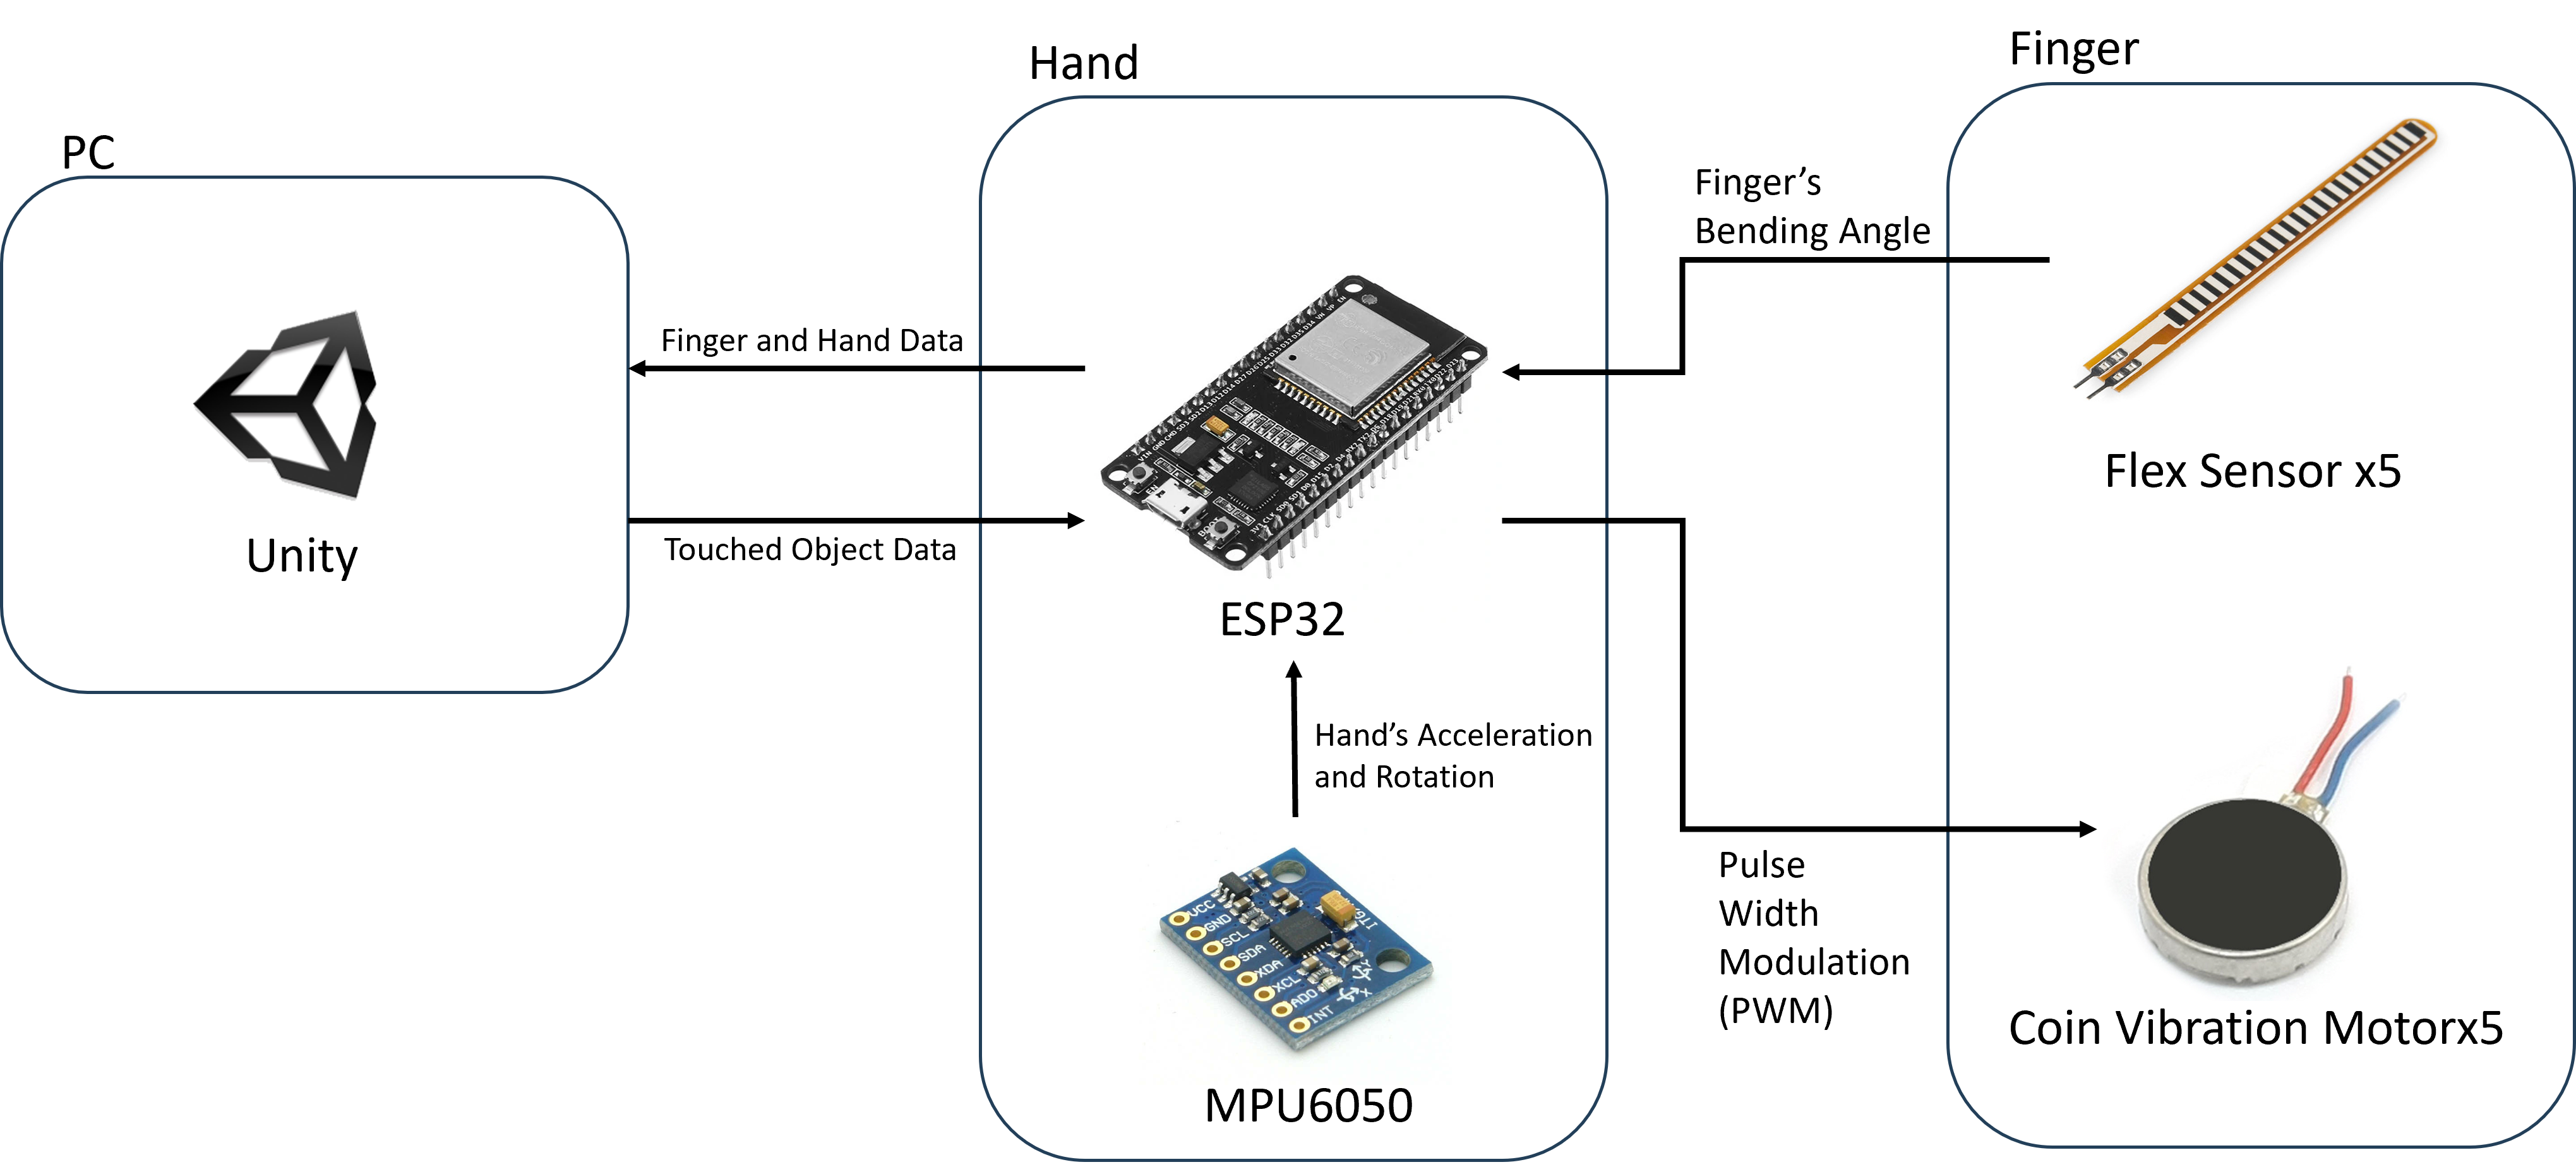
\includegraphics[width=1\textwidth]{Pictures/system_diagram.png}%imagine location
	\caption{System architecture of the wearable haptic glove, showing integration between Unity, ESP32, and hardware components}\label{fig:system_diagram}%use name for ref.
\end{figure}
%%%%%%%%%%%%%%%%%%%%%%%%%%%%%%%%%%

\newpage
\subsection{ESP32 Microcontroller}
The ESP32(Fig.~\ref{fig:esp32}) microcontroller serves as the central control unit for the proposed wearable haptic system. Developed by Espressif Systems, the ESP32 is a dual-core, low-power system-on-chip (SoC) designed for IoT and embedded applications. It offers a compact footprint, integrated Wi-Fi and Bluetooth connectivity, and extensive input/output (I/O) support~\cite{esp32docs}. With its small dimensions (approximately 25.5 mm × 18 mm for the ESP32-WROOM-32 variant), it is highly suitable for integration into wearable devices, where minimizing weight and bulk is essential.

\begin{figure}[H]\centering
	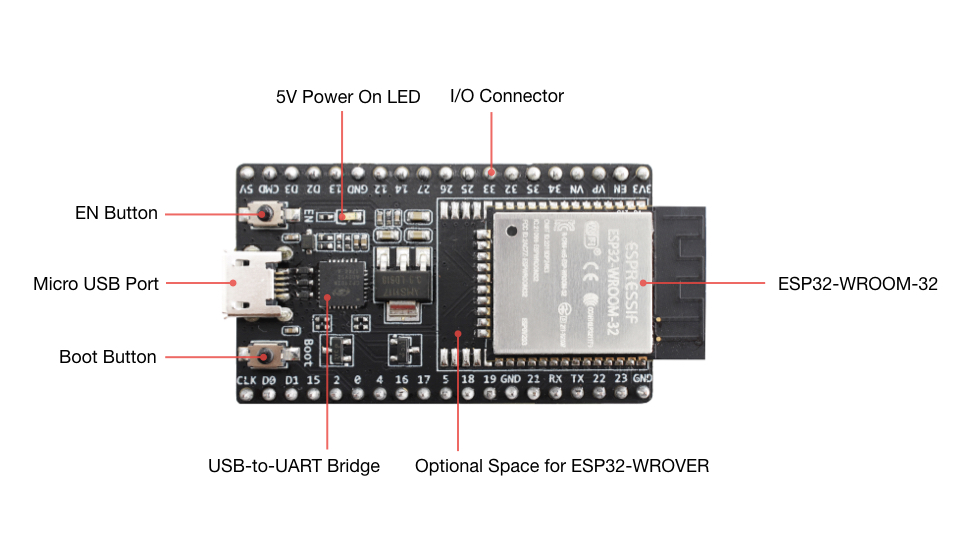
\includegraphics[width=1\textwidth]{Pictures/esp32.jpg}%imagine location
	\caption{ESP32-DevKitC V4 with ESP32-WROOM-32 module soldered~\cite{esp32docs}}\label{fig:esp32}%use name for ref.
\end{figure}

In the proposed system, the ESP32 is responsible for the real-time acquisition of hand motion and gesture data from the sensory module, which includes flex sensors and an inertial measurement unit. It processes these signals and outputs pulse width modulation signals to control a vibrotactile actuator. Additionally, the ESP32 facilitates communication with the virtual reality environment, transmitting hand movement data and receiving feedback commands. This setup supports a low-latency and fully mobile VR haptic interaction system.
%%%%%%%%%%%%%%%%%

\newpage
\subsection{Flex Sensors}
Flex sensors(Fig.~\ref{fig:flex_sensor}) are the key components used to capture finger movements and hand gestures in the proposed wearable haptic device. These sensors are resistive, meaning their electrical resistance changes in proportion to how much they bend. When the sensor bends, the internal conductive particles inside it separate, leading to an increase in resistance. This property allows for direct and continuous analog measurements of finger flexion, facilitating the accurate real-time detection of hand postures.

\begin{figure}[H]\centering
	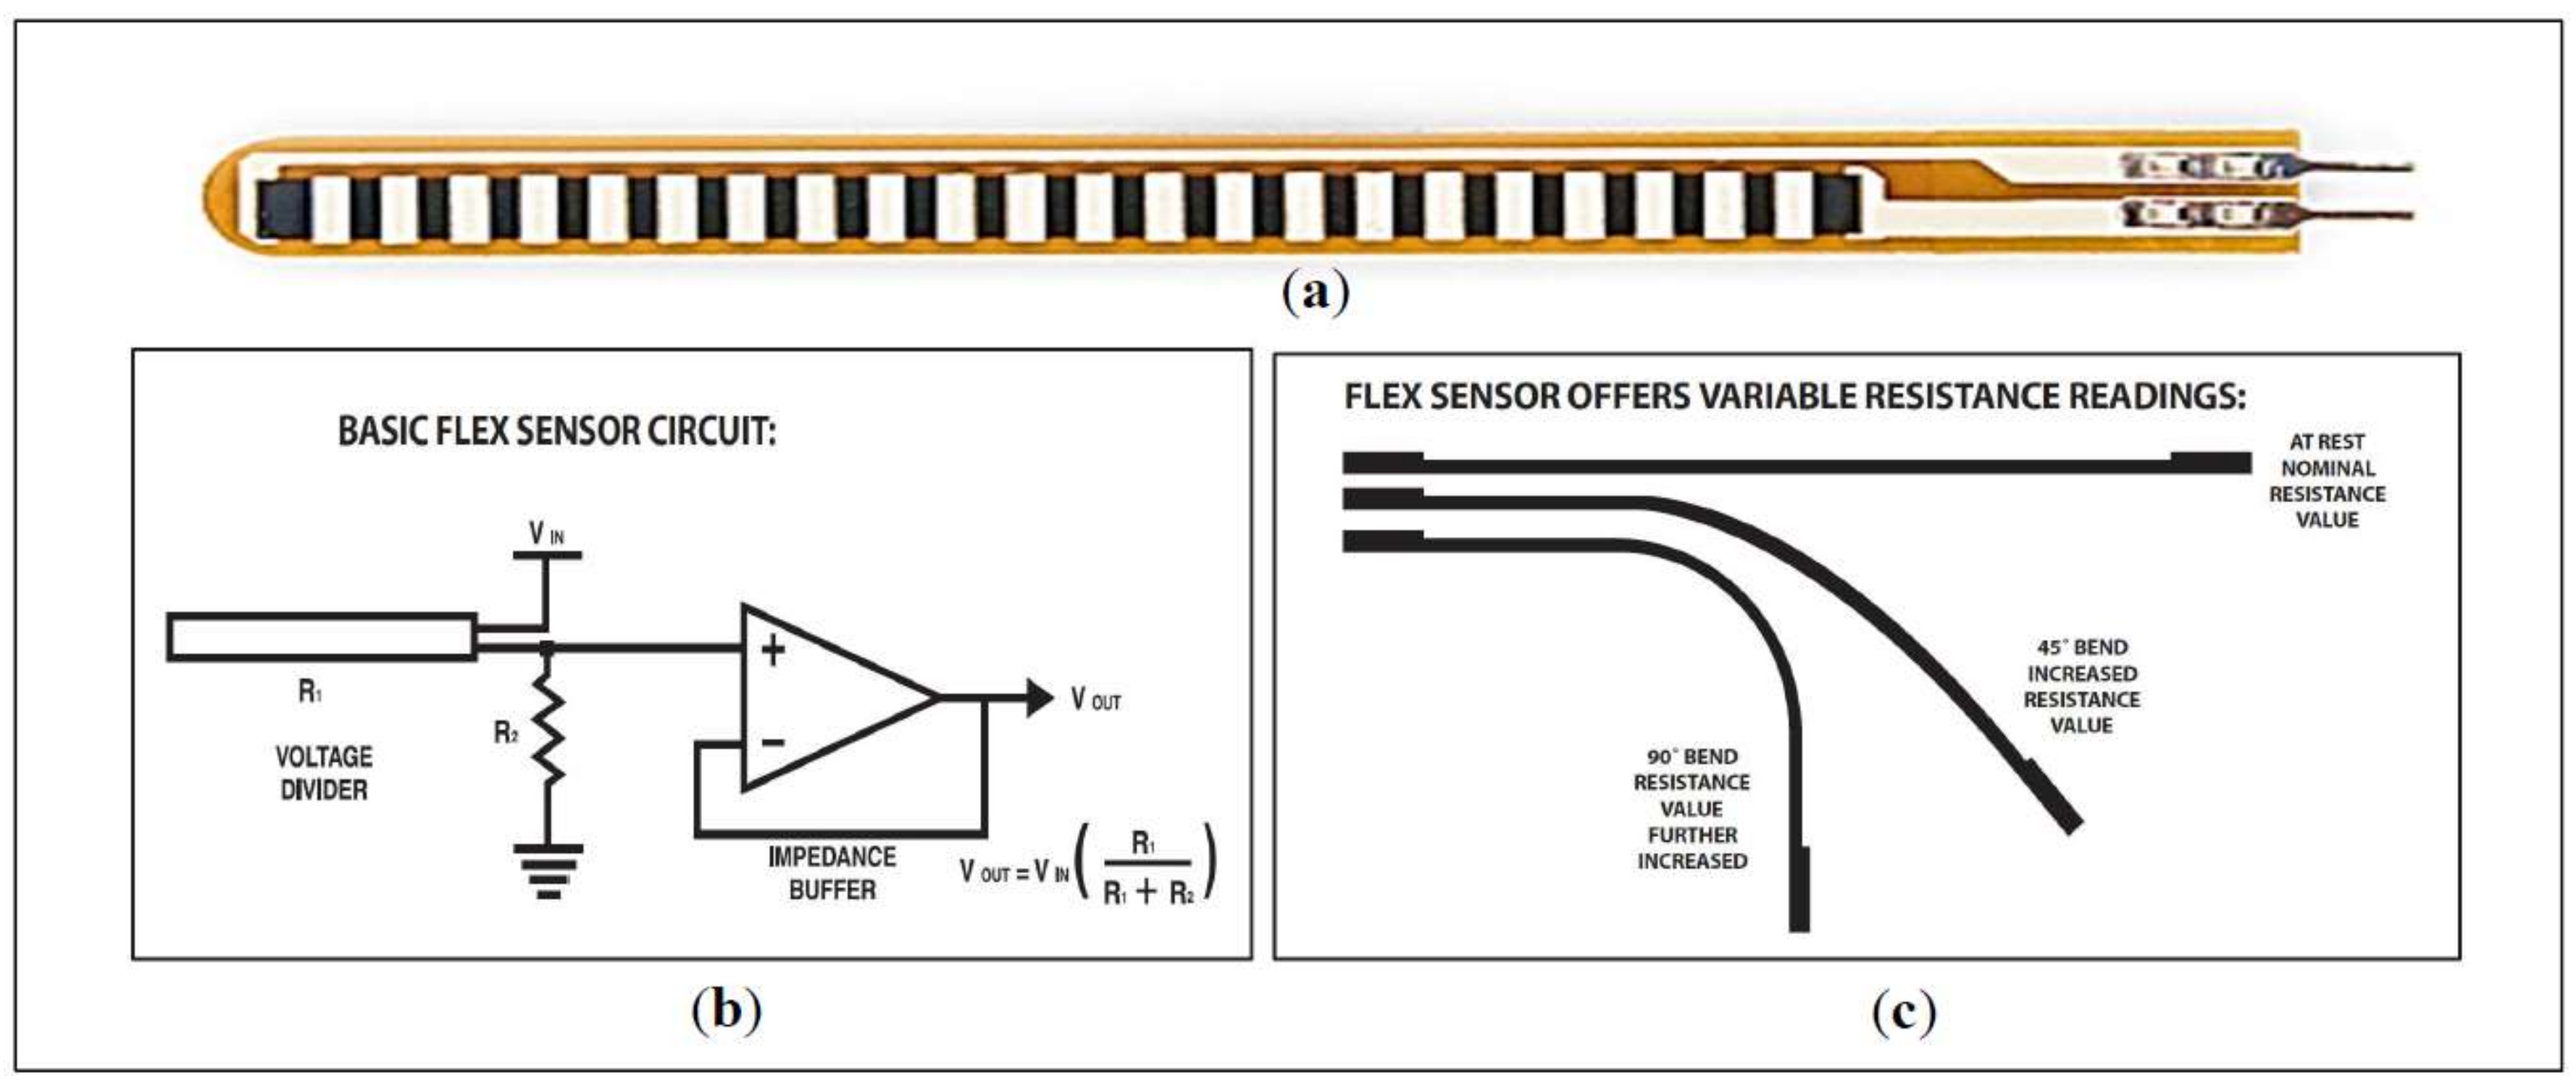
\includegraphics[width=1\textwidth]{Pictures/flex_sensor.png}%imagine location
	\caption{(a) Flex sensor, (b)voltage divider circuit, and (c) flex bend levels~\cite{10.3390/s18072208}}\label{fig:flex_sensor}%use name for ref.
\end{figure}

In this system,  flex sensors are attached along the dorsal side of each finger, from the base to the tip. Each flex sensor is incorporated into a voltage divider circuit, where it acts as the variable resistor. When a user flexes their finger, the corresponding change in resistance causes a drop in output voltage, which is sampled by the 12-bit ADC (Analog-to-Digital Converter) channels of the ESP32 microcontroller as shown in Fig.~\ref{fig:flex_sensor_bend}. This setup allows for precise real-time measurement of finger bending angles, translating physical finger positions into digital signals that can be used for gesture classification and interaction mapping within the VR environment.

\begin{figure}[H]\centering
	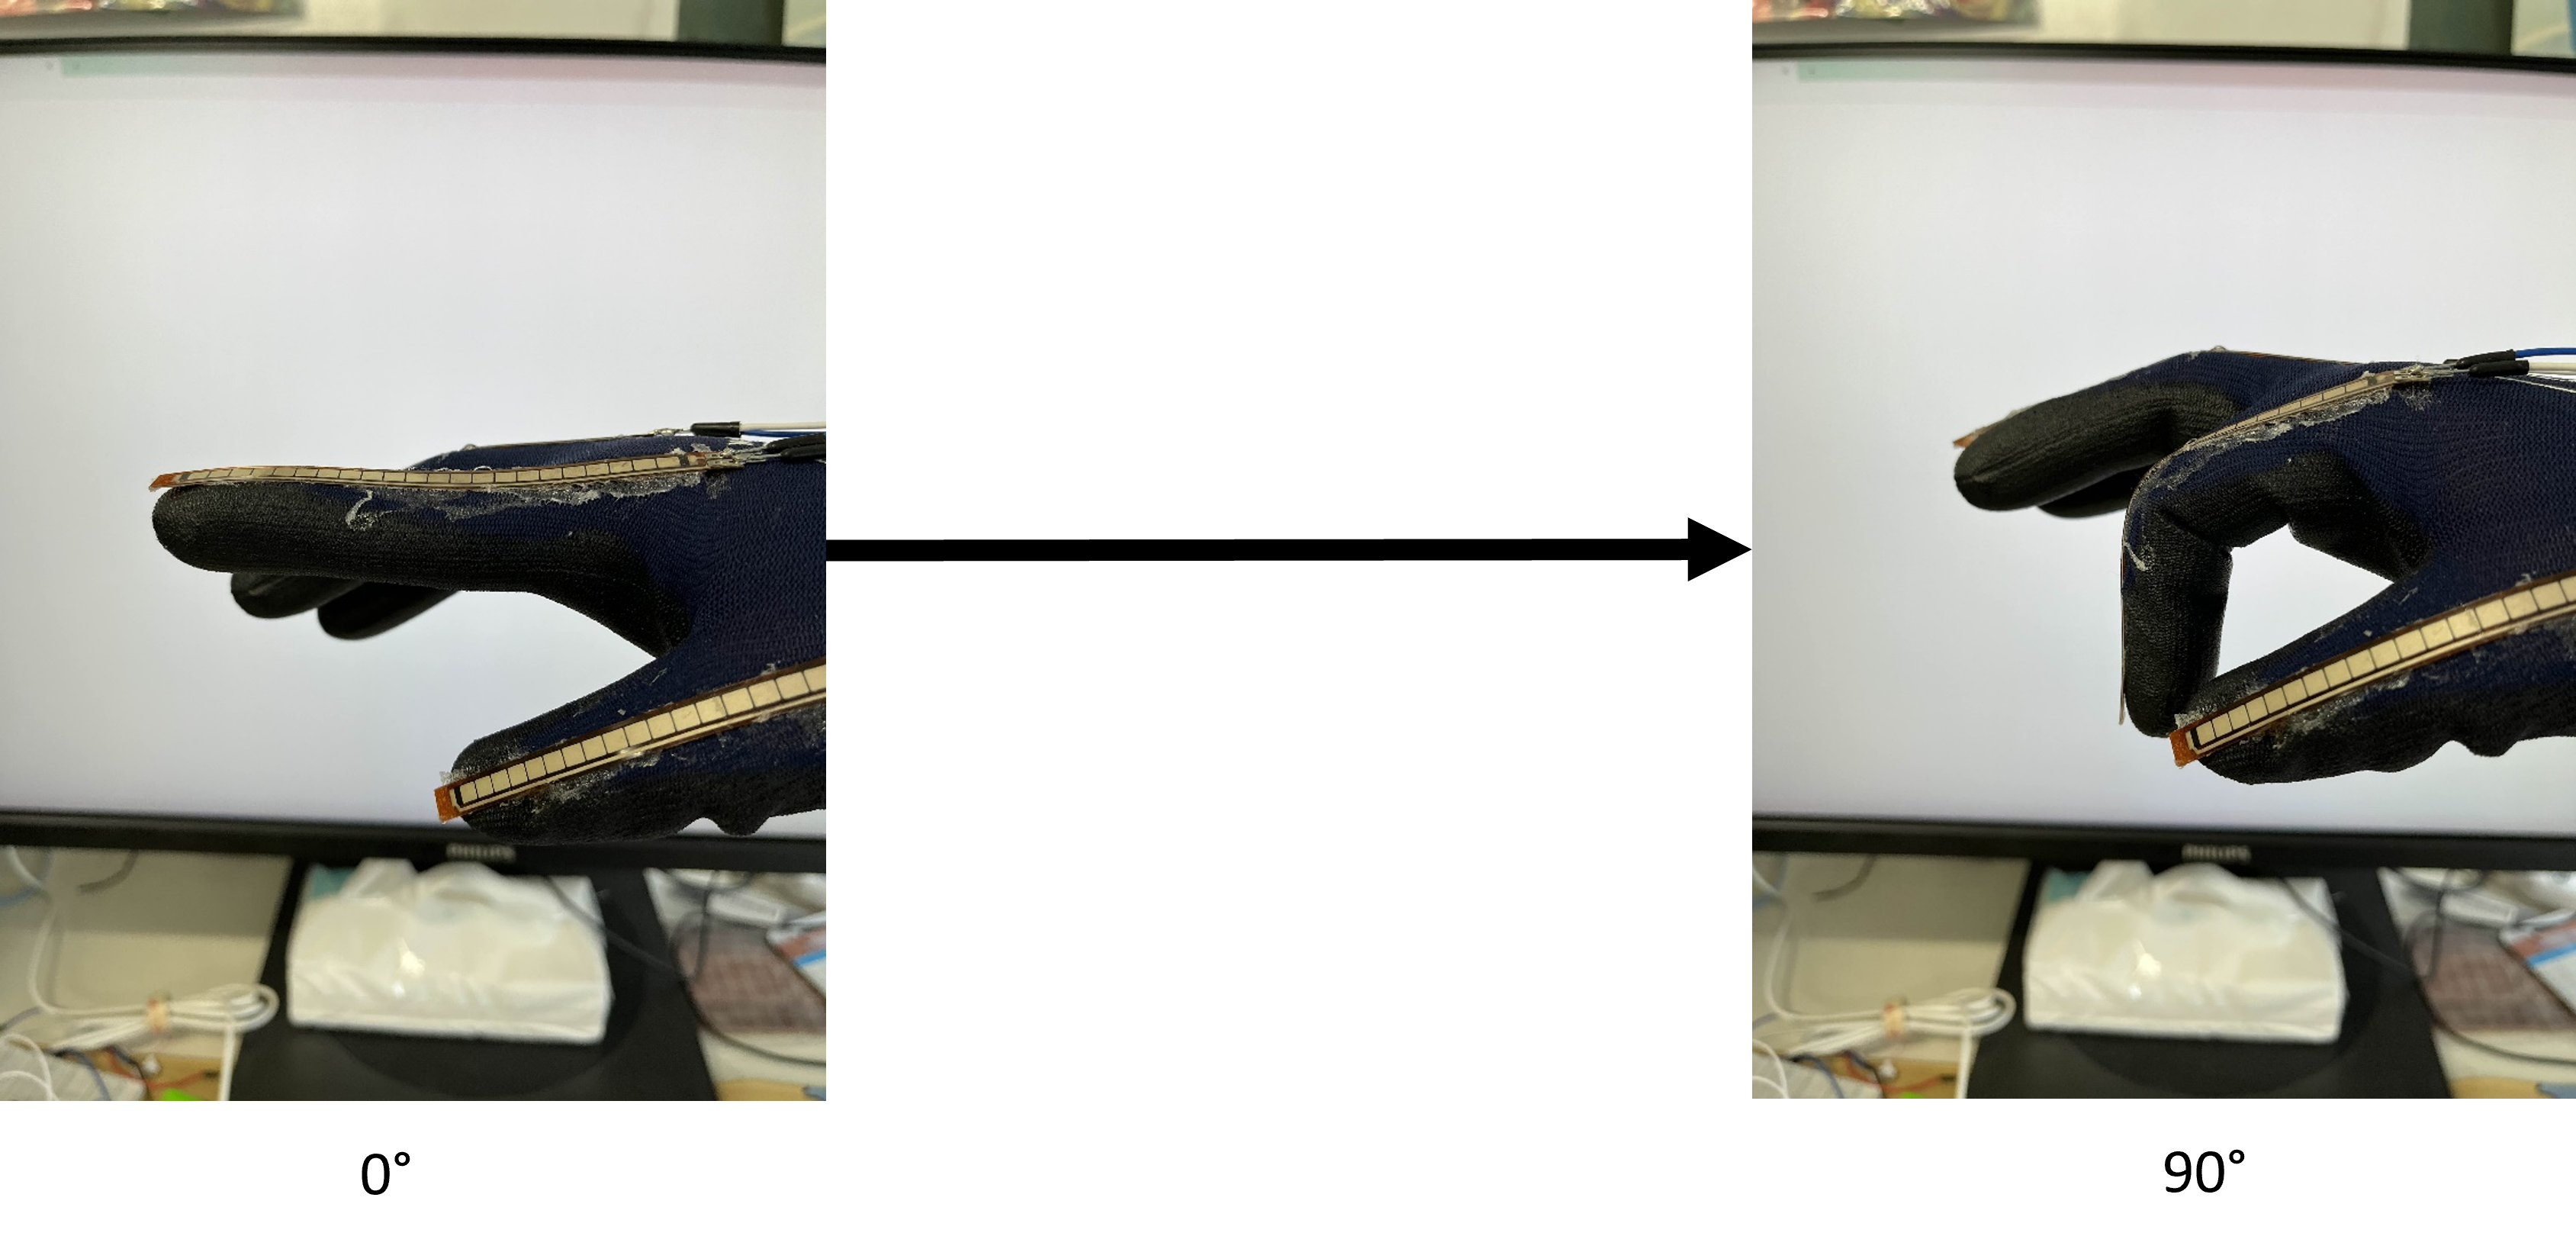
\includegraphics[width=1\textwidth]{Pictures/flex_sensor_bend.png}%imagine location
	\caption{Atteched flex sensor}\label{fig:flex_sensor_bend}%use name for ref.
\end{figure}

One of the main reasons for choosing flex sensors is their compact size, lightweight design, and mechanical flexibility. These features make them ideal for wearable applications as they do not hinder natural hand movements. Unlike vision-based tracking systems, flex sensors do not require external cameras or a direct line of sight, which ensures reliable tracking performance in various lighting conditions and during occluded hand interactions. Furthermore, flex sensors are energy-efficient and only draw a minimal amount of current, which contributes to a longer battery life for wearable devices.

By integrating flex sensors into the proposed device, the system accurately captures detailed finger movements, which are crucial for gesture recognition, interaction triggers, and texture manipulation tasks in virtual reality. The continuous, low-latency data obtained from the flex sensors complements the data from inertial measurement units, creating a multi-modal sensing system that enhances the realism of interactions with virtual objects.
%%%%%%%%%%%%%%%

\newpage
\subsection{Coin Vibration Motor}
The coin vibration motor(Fig.~\ref{fig:coin_motor}), known as the Eccentric Rotating Mass (ERM) type, is used as the main actuator to provide vibrotactile feedback in the proposed wearable haptic device. This type of motor works by rapidly rotating an off-center mass attached to its shaft, which creates oscillations that produce tactile sensations on the skin. Coin motors are favored in wearable devices due to their compact circular shape, lightweight (typically weighing under 3 grams per motor), and straightforward driving circuitry. These features make them ideal for applications where form factor and mobility are crucial design considerations~\cite{coin_motor}.

\begin{figure}[H]\centering
	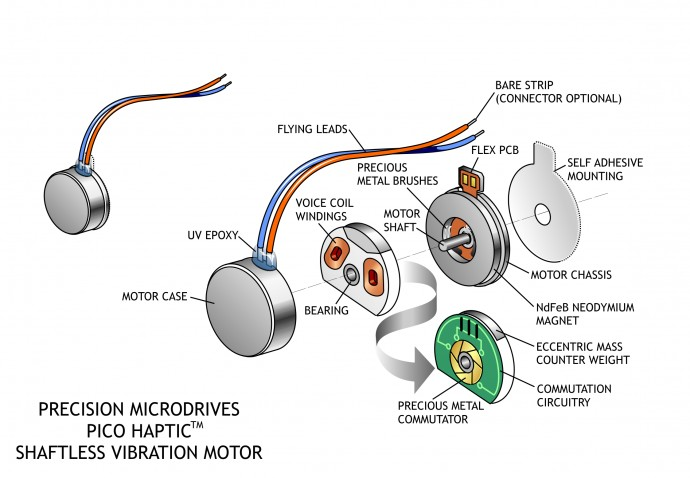
\includegraphics[width=0.7\textwidth]{Pictures/coin_motor.jpg}%imagine location
	\caption{The components of coin vibration motor~\cite{coin_motor}}\label{fig:coin_motor}%use name for ref.
\end{figure}

In this system, as shown in Fig.~\ref{fig:coin_motor_2} 10 mm coin vibration motors that operate at a nominal voltage of 3 V are attached to the fingertip regions of the glove to enhance skin contact and tactile feedback. The motors are controlled using pulse width modulation signals generated by the ESP32 microcontroller. By adjusting the PWM duty cycle and frequency, the system can modulate the intensity and frequency of the vibrations, simulating different levels of surface smoothness or roughness in virtual environments.

\begin{figure}[H]\centering
	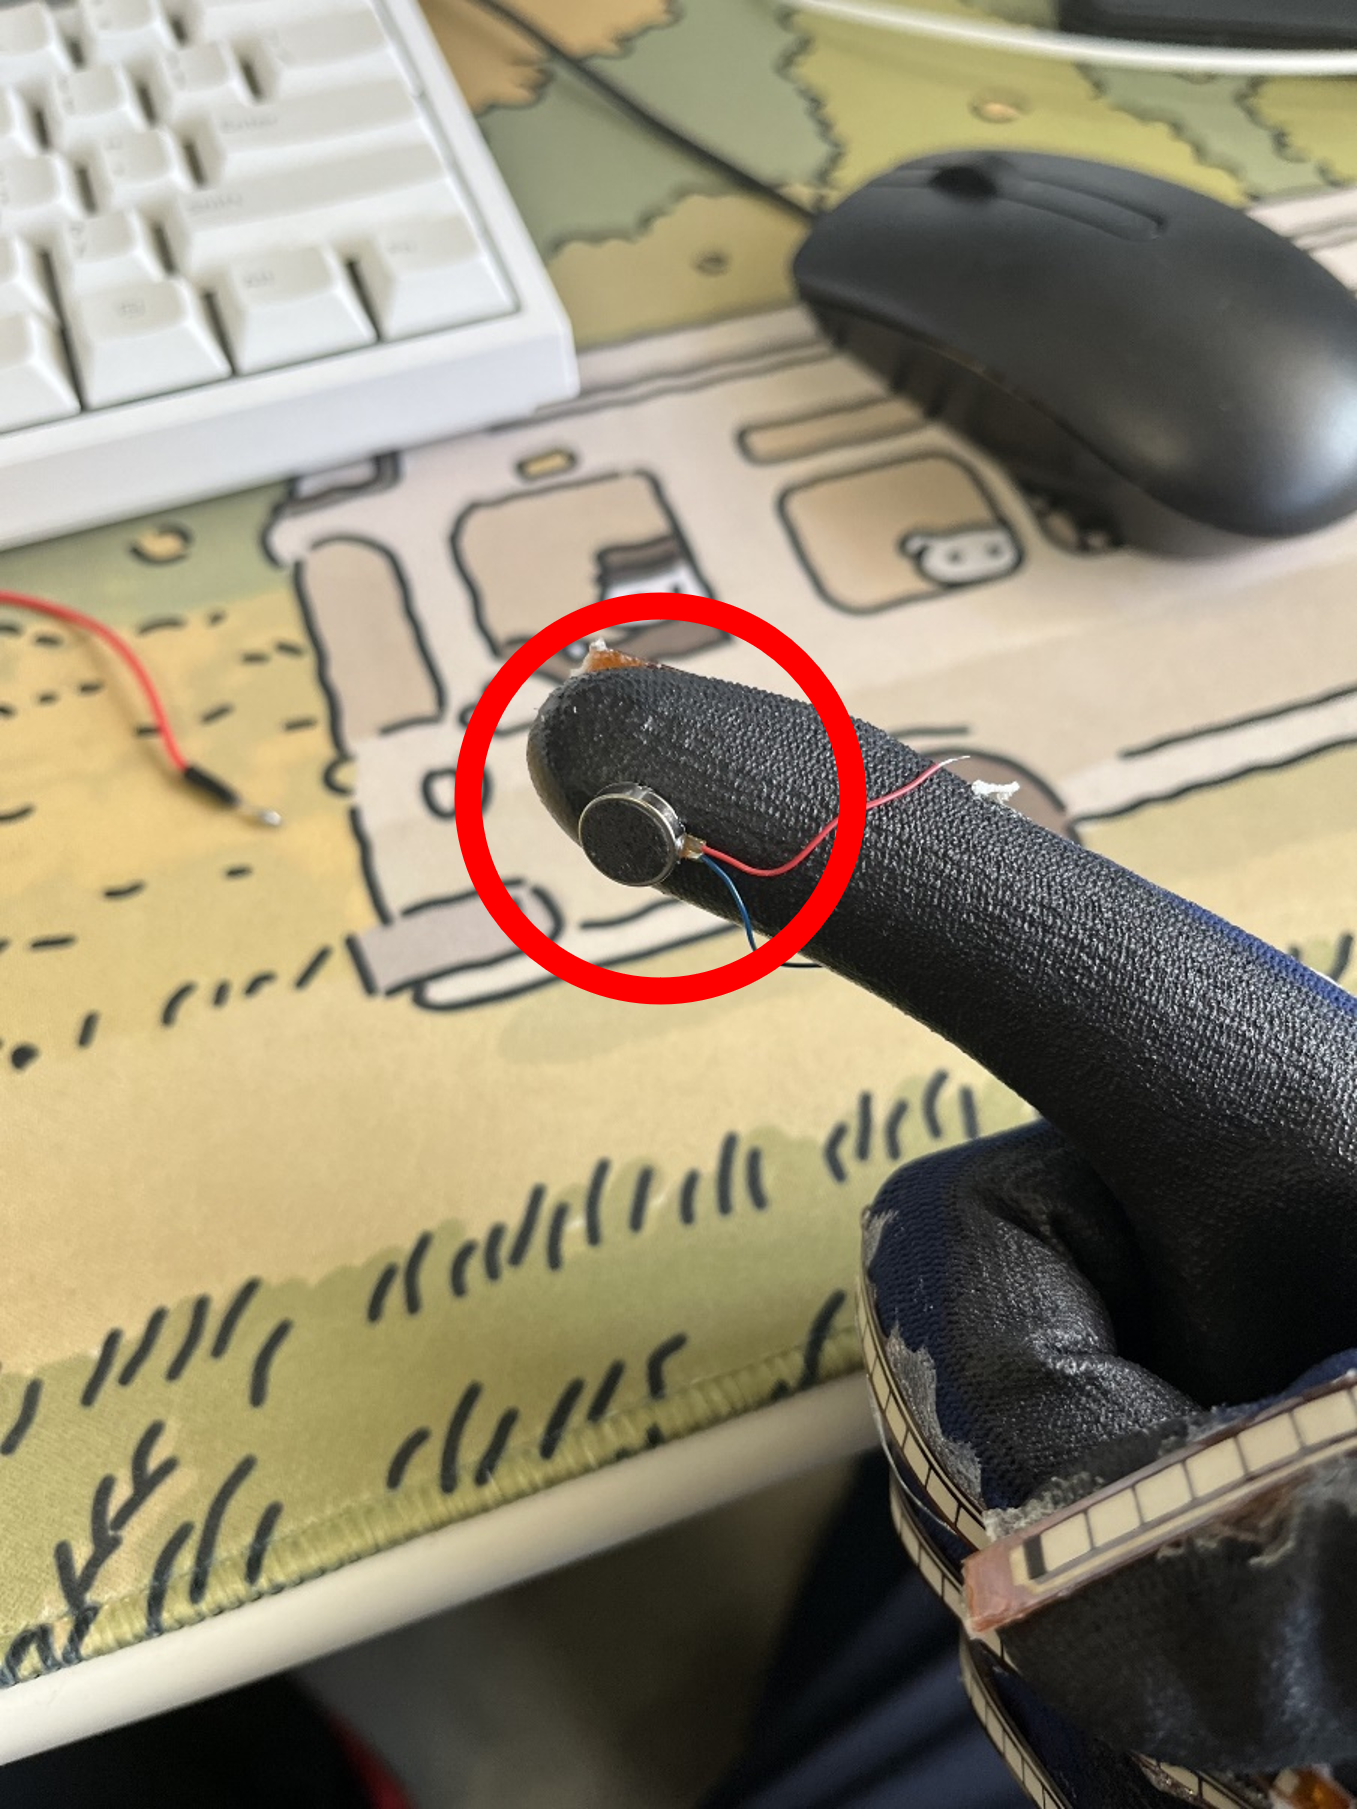
\includegraphics[width=0.5\textwidth]{Pictures/coin_motor_2.png}%imagine location
	\caption{Attached coin motor}\label{fig:coin_motor_2}%use name for ref.
\end{figure}

The selection of coin-type vibration motors in this system is based on four key factors that align with the design goals of portability, simplicity, and effective tactile feedback. Their compact and lightweight design allows for seamless integration into wearable devices without obstructing natural hand movement or causing user fatigue. Additionally, the mechanical simplicity of coin motors enables direct control through pulse width modulation, eliminating the need for complex driver circuits. This makes them easy to integrate with microcontrollers like the ESP32. 

Furthermore, their low power consumption supports prolonged use in battery-powered and untethered VR environments. Finally, coin motors are cost-effective, providing a practical alternative to more complex and expensive actuators while still offering sufficient tactile feedback to convey virtual textures effectively. These combined advantages make coin vibration motors an excellent choice for achieving lightweight, low-latency, and immersive haptic feedback in wearable VR systems.
%%%%%%%%%%%%%%%
\newpage
\subsection{MPU-6050}
The MPU-6050 (Fig.~\ref{fig:mpu}) is integrated into the proposed wearable haptic system to ensure reliable and continuous tracking of hand orientation and movement dynamics. It features a highly integrated 6-axis Micro-Electro-Mechanical  (MEMS) System sensor, which includes both a 3-axis gyroscope and a 3-axis accelerometer in a single, compact module. This combination allows for the measurement of angular velocity and linear acceleration, which are crucial for detecting hand tilting, rotation, and motion trajectories during virtual interactions~\cite{mpu}.

\begin{figure}[H]\centering
	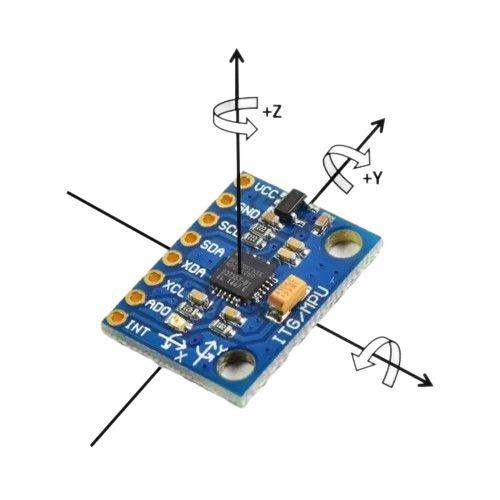
\includegraphics[width=0.7\textwidth]{Pictures/mpu.png}%imagine location
	\caption{MPU-6050~\cite{mpu}}\label{fig:mpu}%use name for ref.
\end{figure}

The MPU-6050 features a compact footprint of 4×4×0.9 mm and low power consumption, making it ideal for wearable systems where minimizing size and energy usage is crucial for comfort and battery life. It connects to the ESP32 microcontroller through the I²C digital interface, which simplifies wiring and makes it easier to integrate into compact glove designs. The device's sampling rate can be configured to a maximum of 1 kHz, enabling high-frequency motion data acquisition that is essential for providing responsive and real-time haptic feedback.

A key feature of the MPU-6050 is its Digital Motion Processor (DMP), an internal processor capable of performing sensor fusion algorithms such as gyroscope and accelerometer data filtering, tilt angle estimation, and motion tracking directly on-chip. This significantly reduces computational overhead on the ESP32 microcontroller, allowing more efficient handling of haptic feedback generation and wireless communication tasks~\cite{mpu6050datasheet}.

In this system, IMU data complements flex sensor data to enhance the fidelity of gesture recognition and dynamic virtual object interaction. By being attached to the glove, the MPU-6050 provides continuous spatial orientation information such as wrist rotation and general hand movement, which cannot be captured by flex sensors alone. This integration ensures more natural and accurate virtual manipulation, especially during dynamic tasks. 

\subsection{Combined Haptic Feedback Device}
In Fig.~\ref{fig:finalglove}, the fully assembled wearable glove system is displayed. This completed device facilitates natural hand gesture recognition while providing vibration-based tactile feedback to the user. It supports real-time interaction in virtual environments by integrating gesture input and haptic output into a compact design. The glove allows users to manipulate virtual objects freely while simultaneously receiving dynamic feedback that corresponds to virtual surface textures. This feature enhances immersion and realism during virtual reality experiences.

\begin{figure}[H]\centering
	\includegraphics[width=0.7\textwidth]{Pictures/glove_1.png}%imagine location
	\caption{Finished glove}\label{fig:finalglove}%use name for ref.
\end{figure}

The final prototype weighs approximately 160 grams, ensuring comfort during extended use. The overall dimensions of the glove, which includes embedded sensors and actuators, are about 250 mm in length and 115 mm in width. The flex sensors can detect finger bending angles ranging from 0° to approximately 150° for each finger, operating at a default sampling frequency of 1000 Hz. The inertial measurement unit captures the hand's angular orientation across three axes—pitch, yaw, and roll—supporting an angular velocity range of ±250°/s and acceleration ranging from ±2g to ±16g, also with a default detection frequency of 1000 Hz.

The vibration feedback is produced using coin vibration motors, which are controlled through pulse-width modulation. These motors deliver cycle rate vibrotactile feedback with a default output update frequency of 5000 Hz, synchronized with contact events in the virtual environment. This setup strikes a balance between a lightweight design, responsive gesture tracking, and realistic vibrotactile feedback, making it suitable for wearable VR applications that focus on texture perception.
